\documentclass[12pt,a4paper]{article}
\usepackage{amsmath,amssymb,amsthm,epsf, graphicx, rotating}
\usepackage{fancyhdr}
\usepackage{subfig}
\usepackage{float}
\graphicspath{ {./images/} }

\pagestyle{empty}
\setlength{\parindent}{0pt}
\setlength{\textwidth}{6.5in}
\setlength{\oddsidemargin}{0in}
\addtolength{\textheight}{1in}

\renewcommand\theenumi{\alph{enumi}}
\renewcommand\labelenumi{(\theenumi)}

\newcommand{\Z}{\mathbb{Z}}
\newcommand{\F}{\mathbb{F}}
\newcommand{\R}{\mathbb{R}}
\newcommand{\C}{\mathbb{C}}
\newcommand{\N}{\mathbb{N}}
\renewcommand\vec{\mathbf}

\pagestyle{fancy}
\fancyhf{}
\fancyhead[LE, RO]{Ryan Liu}

\theoremstyle{definition}
\newtheorem{problem}{}

\author{Ryan Liu}
\title{MATH 442 Homework 9}
\begin{document}

\begin{center}
{\huge MATH 442 \par}
{\Large Homework  9  \par}
{\normalsize Name: Ryan Zhuo Lun Liu \par}
{\normalsize Student Number: 30328141 \par}
{\normalsize Collaborator: Jagjot Jhajj \par}
\end{center}

\begin{problem} \underline{Answer:}
\begin{proof} 
$C_2$, the 2-cycle, is 2-chromatic, 2-chromatic(e), and 2-chromatic(f). \\

As $C_2$ is 2-regular, it is 2-chromatic. As there are only two faces, $C_2$ is 2-chromatic(f). As $C_2$ is 2-regular, which is even, $C_2$ is 2-chromatic(e).

\begin{figure}[H]
    \centering
    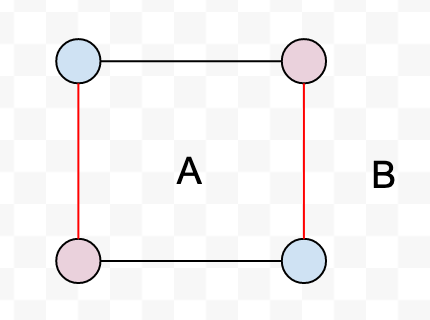
\includegraphics[scale=0.5]{q1.png}
    \caption{Q1}
    \label{fig:my_label}
\end{figure}
\end{proof}
\end{problem}

\begin{problem} \underline{Answer:}
\begin{proof} 
Similar to the idea we for Vizing's theorem in class, we will give colourings to the edges in $Q_k$ according to their orientation. \\

Referring to Figure 2, we can start by colouring the outer edges, starting from $c_1$, and moving in a clockwise pattern and returning to $c_1$ after we have used $c_k$. For any inner edge $u$, colour it the same colour as a parallel outer edge $v$. \\

This pattern only works as each vertex in $Q_k$ is connected to a vertex that differs in a single digit. This property prevents a cycle of odd length from existing, and thus can be coloured like so. Thus, $\chi'(Q_k) = k$

\begin{figure}[H]
    \centering
    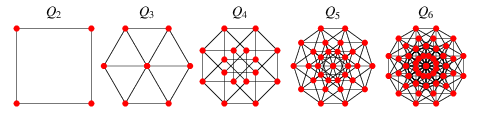
\includegraphics[scale=0.6]{q2.png}
    \caption{Several Hypercubes}
    \label{fig:my_label}
\end{figure}
\end{proof}
\end{problem}

\begin{problem} \underline{Answer:}
\begin{proof} 
Vizing's Theorem states that $\chi'(G) = d + 1$ or $d$. Now suppose that for a graph $G$ that is $d \geq 2$ regular with odd number of vertices, $\chi'(G) = d$. \\

Since we can colour the edges with only $d$ colours, let's consider $c_1$, one of the $d$ colours. Since every vertex has degree $d$, every vertex must have an edge of colour $c_1$. Since every edge is incident to two vertices, and there must be an even number of vertices in $G$, where each is incident to an edge of every colour from $c_1$ to $c_d$. However, our assumption states that $G$ has an odd number of vertices. Thus, $\chi'(G) \neq d$ and by Vizing's Theorem, $\chi'(G) = d + 1$.
\end{proof}
\end{problem}

\begin{problem} \underline{Answer:}
\begin{proof} 
This configuration would require 6 lecture periods. \\

Referring to Figure 3, we see that vertex $b$ has the highest degree, 5. We can calculate the chromatic polynomial starting from here, and assign $k$ to $b$, $k - 1$ to $e$ and $g$, $k - 2$ to $a$, $k - 3$ to $c$, $d$, and $f$.

Multiplying these terms up gives us: $P_G(k) = (k)(k - 1)^2(k - 2)(k - 3)^3$. This means that $\chi'(G) = 4$ as it is the smallest $k$ such that $P_G(k) \neq 0$.

\begin{figure}[H]
    \centering
    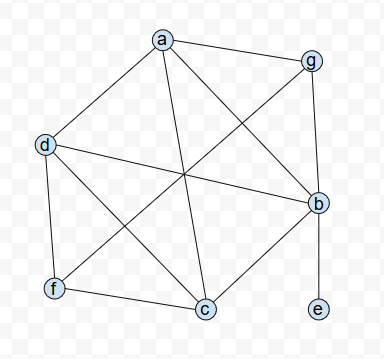
\includegraphics[scale=0.5]{q4.png}
    \caption{Q4}
    \label{fig:my_label}
\end{figure}
\end{proof}
\end{problem}

\begin{problem} \underline{Answer:}
\begin{proof} The statement that a simple connected graph $T$ is a tree iff adding an edge between two existing vertices of $T$ creates exactly one cycle will be proved both ways.

$\rightarrow$: \\
Let $v$, $w$ be two vertices in $T$. Since $T$ is a tree, there exists exactly one path between $v$ and $w$. Adding an edge between $v$ and $w$ creates at least one cycle. Let's suppose that this created at least two cycles. \\

Since we created two cycles, this new edge $e$ must exist in both cycles. Now remove $e$ from both cycles and we see that now there are two paths from $v$ to $w$. This is a contradiction as $T$ is a tree and there is exactly one path from $v$ to $w$. Thus, if $T$ is a tree, then adding one edge between two existing vertices creates exactly one cycle.

$\leftarrow$: \\
In order for $T$ to create a cycle when connecting two vertices by an edge, $T$ must be connected. However, $T$ must also not have an existing cycle as we can connect any two vertices in the cycle to create an additional cycle, contradicting the claim that we would create exactly one cycle. Thus, $T$ is connected and does not have any existing cycles, so $T$ must be a tree.
\end{proof}
\end{problem}

\begin{problem} \underline{Answer:}
\begin{proof} Let's first consider the formula for the average degree $a$ as a function of the number of vertices $v$. \\

Lemma: The average degree $a$ can be represented by $a = \frac{2v - 2}{v}$. This will be proved by induction on the number of vertices $v$. \\

\underline{Base Case:} $v$ = 1 and the lemma states $\frac{2 - 2}{1} = 0$ \\

\underline{Inductive Step:} Suppose the lemma is true for all $v < n$ and let $T$ be a tree with $n$ vertices. \\

Let $x$ be a leaf in $T$ and remove it from $T$. $T - x$ has $n - 1$ vertices and we can apply the inductive hypothesis and the average degree of $T - x$ is $\frac{2n - 4}{n - 1}$. The sum of degrees of all vertices in $T - x$ is $2n - 4$ as indicated by the inductive hypothesis. Now let's add $x$ back in. The sum of degrees increases by $2$, one from $x$ and one from the vertex incident to $x$, so now the average degree is $\frac{2n - 2}{n}$. Thus, $a = \frac{2v - 2}{v}$. \\

As we have proven the lemma, we can rearrange the formula to instead tell us the number of vertices as a function of the average degree. This gives us $v = \frac{2}{2 - a}$. Alternatively, we could say that that a tree with $n$ vertices has $n - 1$ vertices, and the sum of degrees is twice the number of edges, we can say that the average degree is $\frac{2(n - 1)}{n}$ or $\frac{2v - 2}{v}$.
\end{proof}
\end{problem}

\begin{problem} \underline{Answer:}
\begin{proof} 
Using the answer to Q6, we see that the the average degree of a tree must be $< 2$. \\

Suppose $T$ has as many leaves as non-leaf vertices and that every non-leaf vertex has degree of at least 3. This configuration would not be possible as the average degree of a tree must be $< 2$. Adding a non-leaf vertex would increase the degrees by 3, as 1 is a leaf and 2 is not allowed. This would increase the average degree as well. Thus, we have arrived at a contradiction, and $T$ must have more leaves than non-leaf vertices. 
\end{proof}
\end{problem}
\end{document}
